\documentclass[12pt,a4paper,notitlepage]{report}
\usepackage[utf8]{inputenc}
\usepackage{amsmath}
\usepackage{amsfonts}
\usepackage{amssymb}
\usepackage{graphicx}
\usepackage{cite}
\usepackage{url}

\usepackage{caption}

\usepackage[toc,page]{appendix}
\usepackage{hyperref}

\usepackage[left=2cm,right=2cm,top=2cm,bottom=2cm]{geometry}
\title{}
\author{}
\date{}
\begin{document}

\chapter*{Literature Review}

\section*{Tracking user movement}

An obvious way to track user position is to perform double integration on the obtained acceleration to get distance travelled. However this results in introduction of error due to being only an approximation of the underlying signal. Furthermore, integration of the noise component leads to the standard deviation of the error in position increasing with integration time~\cite[p.73]{integrationError}. Thong, Y. K., et al.~\cite{integrationErrorPractical} analysed the practical effect that double integration of accelerometer noise has on this error by carrying out experiments using two commercial accelerometers, and found that this error very quickly accumulates with time~\cite[p.1168]{integrationErrorPractical}. Hence this approach is unsuitable for a navigation system which continuously and precisely requires the user’s current position. Foxlin, E.'s approach~\cite{foxlin2005pedestrian} alleviates the integration error by using the concept of `zero-velocity updates (ZUPTs)’, which exploits the fact that there is a momentary stationary period of zero velocity and acceleration during walking motion when the user’s foot makes contact with the ground. This allows correction of the velocity error after each stride and makes the error accumulation ``linear in the number of steps''~\cite[p.38]{foxlin2005pedestrian}. This however, requires a dedicated sensor to be placed on the user’s foot and does not come under the purview of a smartphone based approach. 


Most dead-reckoning systems thus make use of step detection to identify user movement and step length estimation to estimate their displacement and avoid the double integration problem. Existing approaches that make use of a smartphone’s inertial sensors typically restrict the phone’s position to two scenarios - the user having the phone in their pocket and/or in front of them in their hand. Steps are detected by identifying the consistent change in sensor readings, particularly the accelerometer, caused by rythmic motion during walking. For instance, Wang, H., et al.~\cite{wang2012no} observe that the graph of magnitude readings of a 3-axis accelerometer follow a sinusoidal pattern corresponding to the ``natural up/down bounce of the human body for each step taken''~\cite[p.203]{wang2012no} in both the in-hand and pocket case. They then isolate individual steps through simple peak detection and thresholding in the graph. Li, F., et al.~\cite{li2012reliable} also use accelerometer magnitude in a similar manner to identify steps, subsequently applying heuristic constraints and dynamic time warping validation to reduce false positives.  

While taking the magnitude of the accelerometer allows the step detection procedure to be independent of the phone’s orientation, as a side effect moving the phone along the axes that do not correspond to the user’s vertical movement can also produce similar sinusoidal patterns. Jin, Y., et al.~\cite{jin2011robust} isolate acceleration specifically along the required vertical axis by projecting the acceleration measurements from the phone’s local x-y-z axes to the East-North-Up (E-N-U) world co-ordinate system, where `Up' is the desired axis.  This is achieved by using the `rotation matrix' containing orientation measurements that are applied to the acceleration vector in the local co-ordinates. Once the accelerometer readings are obtained on this vertical axis they detect steps by identifying sequences of local maximas followed by local minimas along with thresholding on both the time elapsed and absolute value difference between the two. 

Efforts have also been made to extend step detection to work in arbitrary phone positions, so that it can be used in real-world situations where the position varies as the user performs a multitude of activities. Such approaches either involve broadly identifying the type of activity the user is performing and then using the appropriate sensors for step detection in that particular situation, or generating and using one or more measures that already take into account the variations in position. Susi, M., et al.~\cite{susi2013motion} specify a set of possible user activities and associate with each one unique features based on measures derived from accelerometer and gyroscope readings. The user’s current activity is then identified by extracting the feature set corresponding to their motion and using a pre-defined decision tree to classify it as one of the specified activities. A specific version of the algorithm optimised for peak detection in the context of that particular activity is then used to detect steps. For instance, if the activity is classified as `phone in swinging hand' then gyroscope readings are also considered due to periodic rotation of the user’s arm. Conversely, activities such as texting do not involve any rotation and thus only accelerometer readings are looked at. Zeng, Q., et al.~\cite{zeng2015novel} proposed a novel step counting algorithm that works irrespective of the phone’s position and step mode (variation in the user’s motion, including walking and running). In addition to the accelerometer they also make use of the 3-axis gravity sensor, which provides acceleration acting on each of the axes specifically due to gravity. A change in these values signifies a change in the position/orientation of the phone and can be used to compensate for the resulting variance in accelerometer readings. Thus the authors take a linear combination of the accelerometer and gravity readings to produce a single metric incorporating this compensation, on the basis of which step detection is carried out. Lee, H., et al.~\cite{lee2015step} consider both the short and long term changes in accelerometer magnitude to capture the variations caused due to different positions and step modes. Peak/valley candidates are identified on the basis of measures that track these short/long term changes such as mean and standard deviation. Candidates are then validated using adaptive thresholds which ensure that sufficient time, corresponding to the estimated minimum duration between subsequent steps in standard motion, has elapsed between adjacent peaks and valleys. 

\chapter*{Step Detection}

Step detection is one of the most vital components of the navigation system as it is the basis on which a user's motion is detected. In a dead-reckoning system a user's current position is determined by incrementally estimating their displacement from a previously known position. Thus if the user's starting location is known, step detection along with the user's bearing can be used to identify when they have moved and along which direction. Combining this with step length estimation allows for determining the magnitude of this displacement, which enables keeping track of the user's position as they navigate within the mapped area. 

Algorithms for step detection using smartphones typically analyse the phone's sensor readings and relate them to the user's movement. Deciding on which specific sensors to analyse and the algorithms to apply on them is dependent on the exact placement of the phone while the user walks. The two situations commonly considered are the `in-pocket' case, where the phone is kept in the user's pant pocket near hip level and the `in-hand' case, where the user keeps the phone in their hand and directly in front of them at around chest level. 

Considering that step detection in this project is to be used in the context of a navigation system, the in-pocket case would only be useful to consider if our application was equipped to provide directional information in the form of audio updates, as the user would not be able to observe the phone's screen in this scenario. Our application provides navigation instructions in image and textual format only and hence the in-pocket case is not accounted for. We focus specifically on the in-hand case, which is the most common way in which outdoor navigation applications such as Google Maps are used on smartphones as users have the screen in front of them throughout in order to observe their movement on the map and follow the path provided by the navigational system. Thus our step detection method is also designed to work specifically for the in-hand scenario, and might not operate correctly if the phone is kept in some other position.  

\section*{Sensors Considered}

Existing approaches predominantly make use of the phone's accelerometer readings in order to detect the user's steps. As the name suggests, an accelerometer is a device that measures the acceleration that is applied to the device. In smartphones, this acceleration $A_{d}$ is measured using the relation in 
Equation~\ref{eq:accelerometerAcceleration}~\cite{accelerometerAcceleration}.  

\begin{equation}\label{eq:accelerometerAcceleration}
A_{d} = - \sum F_{s}/massAccelerometer
\end{equation}
\\
where $\sum F_{s}$ is the sum of the forces acting upon the device. Included in $F_{s}$ is the force acting on the device due to the Earth's gravity, which produces acceleration having a constant magnitude of $9.81 m/s^2$. 

In particular, most modern smartphones come equipped with a `3-axis' accelerometer, which reports the accelerations acting separately on the 3 principal axes of the phone's co-ordinate system - X, Y and Z. In Android and iOS these 3 axes are defined relative to the phone's screen when held in its `natural orientation', which is portrait in most cases. The axes are illustrated in Figure~\ref{fig:axisDevice}

\begin{center}
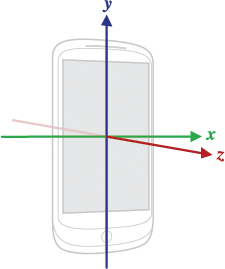
\includegraphics[scale=0.5]{images/axisDevice.png}
\captionof{figure}{The 3 principal axes of smartphones, defined with respect to the screen in its `natural orientation'~\cite{axisDevice}}
\label{fig:axisDevice}
\end{center}

As seen from the figure, the X-axis passes through the side of the phone, the Y-axis is along the vertical segment while the Z-axis projects out from the center of the screen. The positions of these axes remain fixed with respect to the screen, and thus rotate accordingly along with change in the phone's orientation. 


In order to confirm that the actual sensor readings correspond to the described behaviour the logging application was made use of in order to record and analyse the accelerometer data. The first recording was performed with the phone remaining stationary throughout and kept flat on the surface with the screen facing upwards. The readings obtained are shown in Figure~\ref{fig:accelerationZ}.

\begin{center}
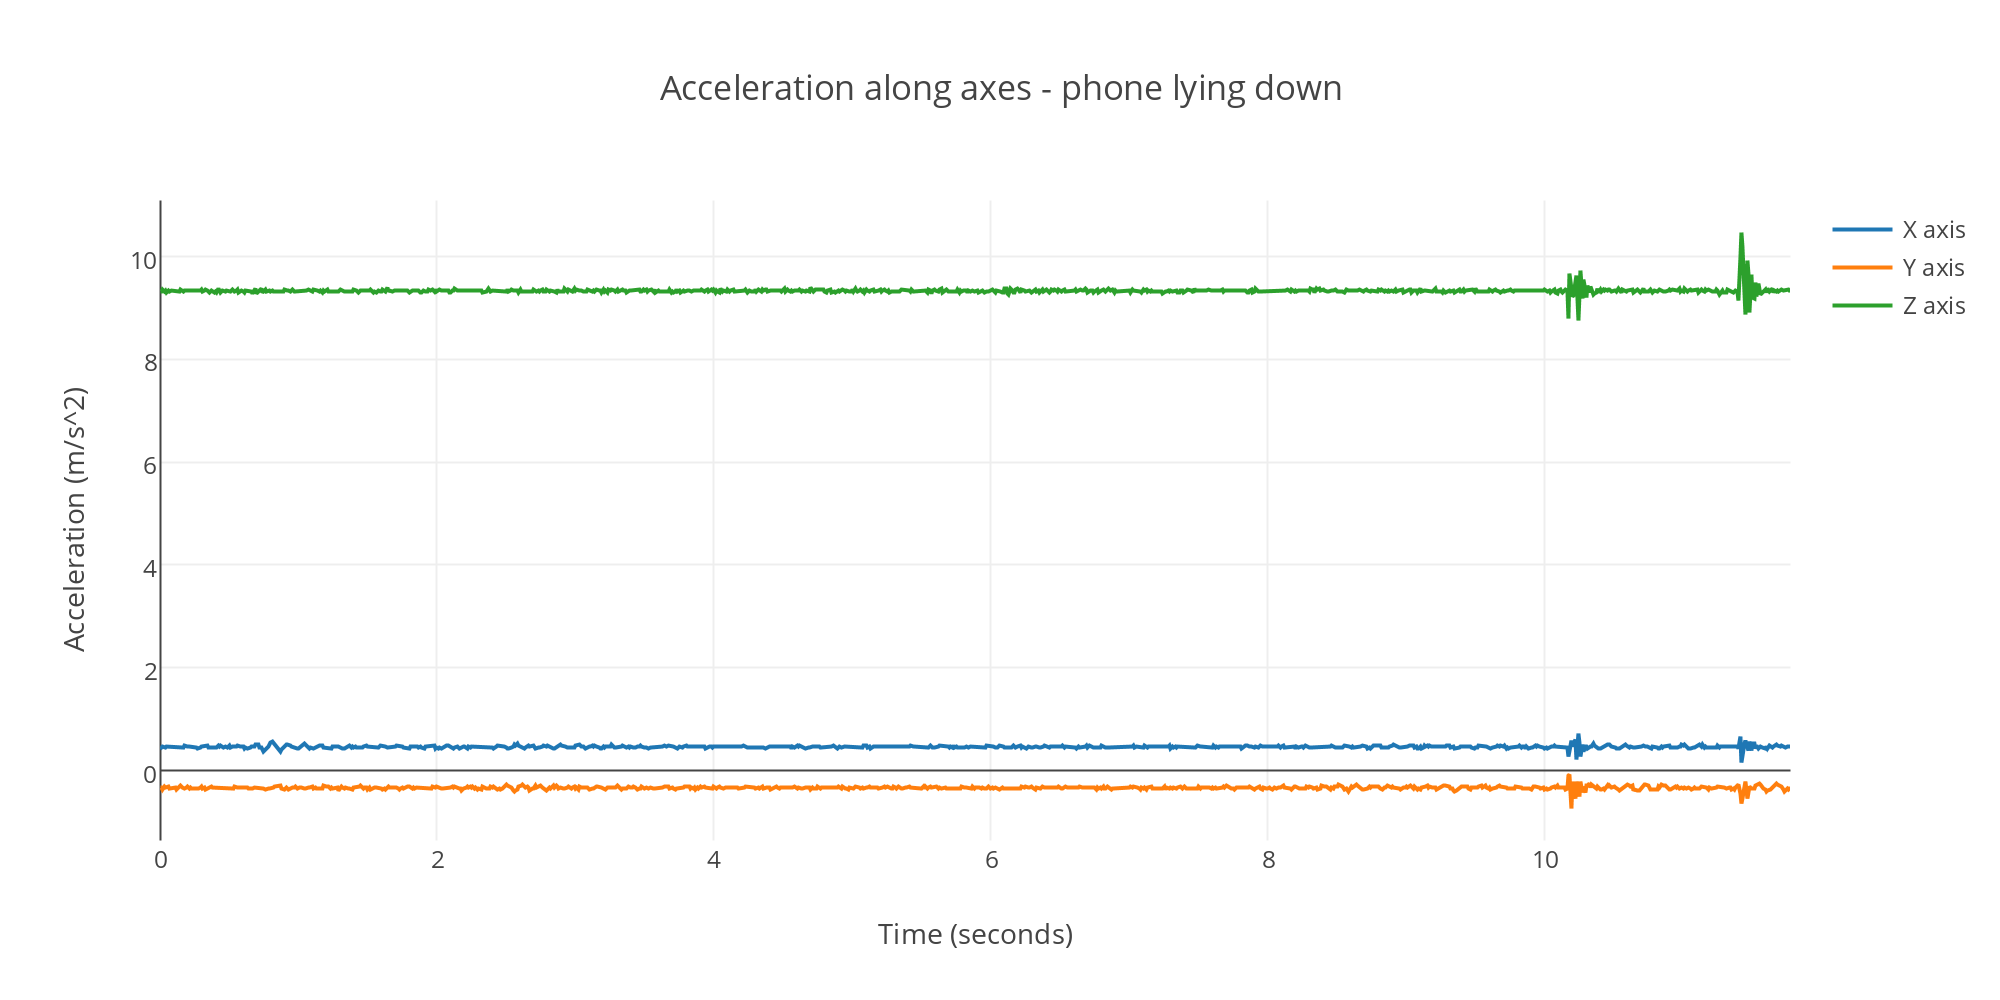
\includegraphics[scale=0.9]{images/accelerationZ.png}
\captionof{figure}{Accelerometer readings with phone kept flat on the surface}
\label{fig:accelerationZ}
\end{center}

As expected, the acceleration along the X and Y axes are close to 0, while there is a constant acceleration of about $9.81 m/s^2$ along the Z axis due to the force of gravity acting downwards through the screen of the phone. Note that the direction of acceleration in this case is upwards as the phone at rest accelerates upwards with respect to the local reference frame of a freely falling object close to the surface. 

This process is repeated with the phone held upright this time (with the bottom of the phone in contact with the surface). The obtained readings are shown in Figure~\ref{fig:accelerationY}.

\begin{center}
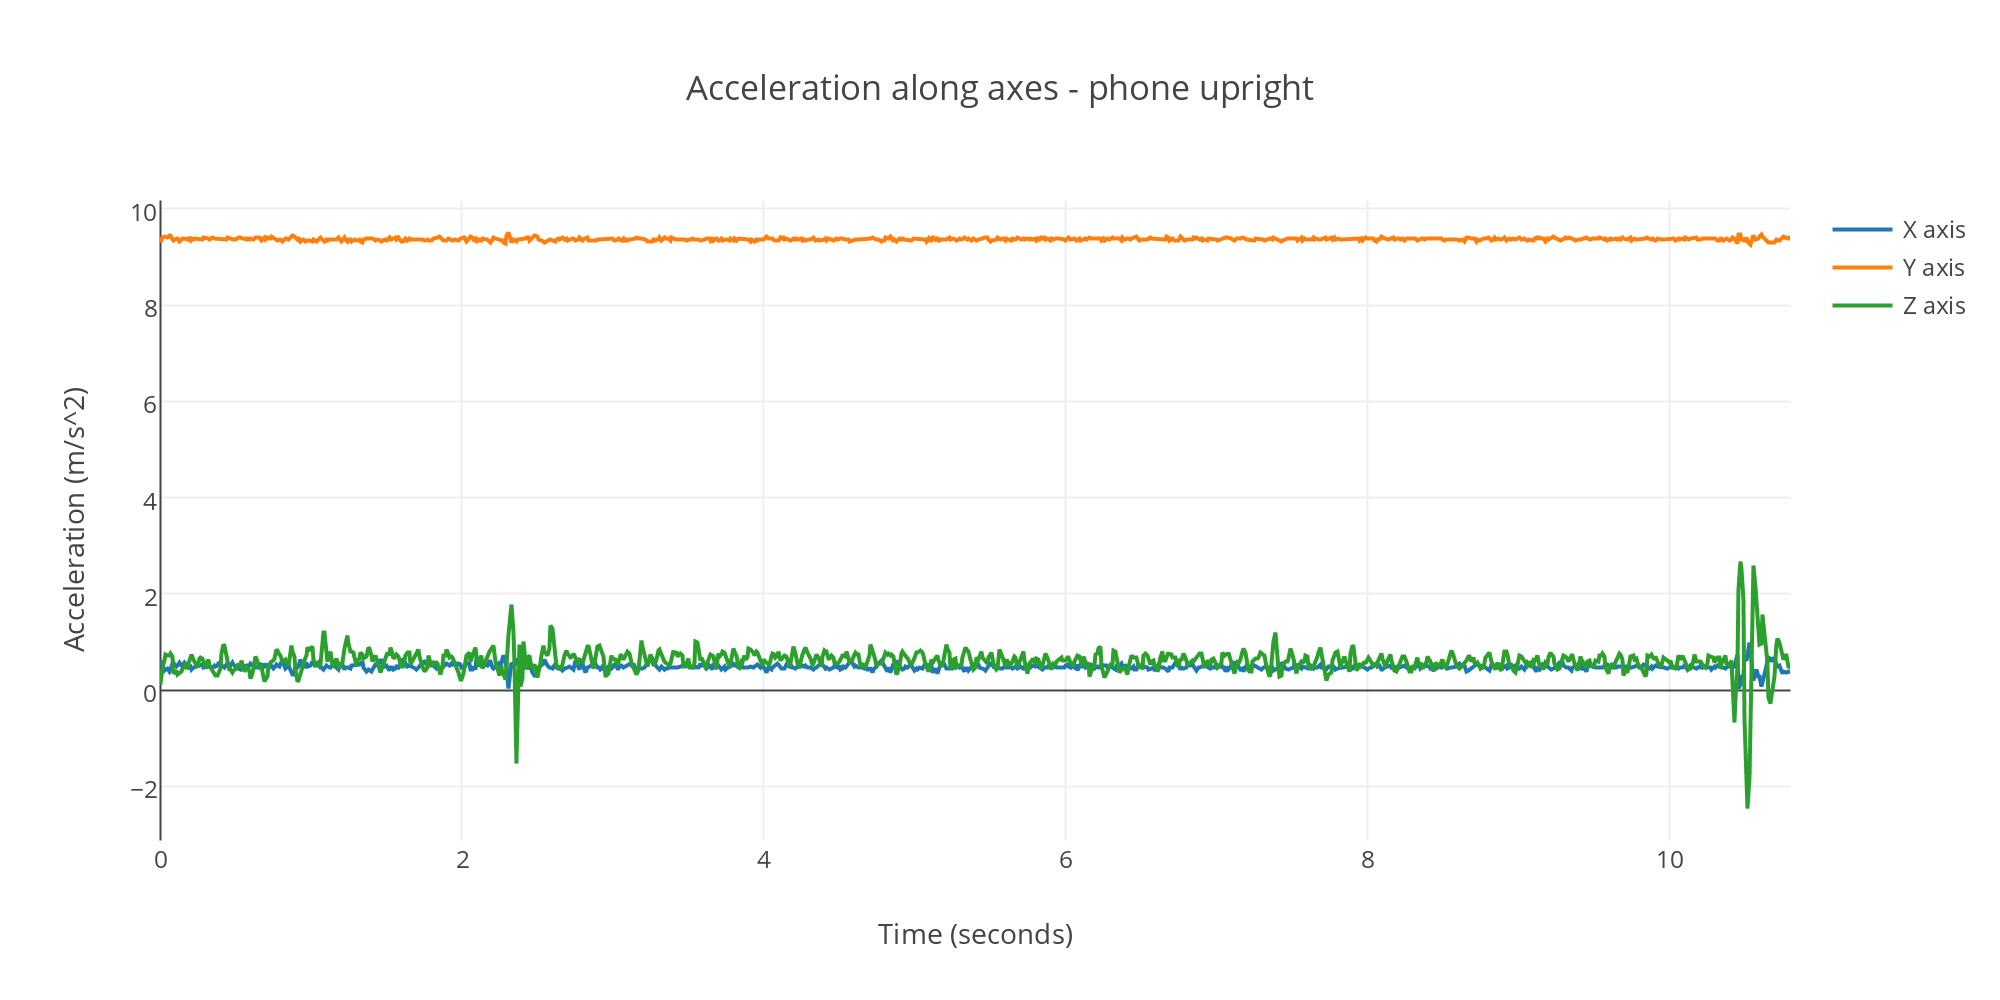
\includegraphics[scale=0.9]{images/accelerationY.png}
\captionof{figure}{Accelerometer readings with phone kept upright}
\label{fig:accelerationY}
\end{center}

The acceleration due to gravity is now along the Y-axis in accordance with the described behaviour, with the momentary spike in the Z-axis acceleration towards the end occurring due to slight movement of the hand while keeping the phone upright. On this basis it can also be concluded that keeping the phone lying on its side would make the gravity acceleration act along the X-axis, showing that the readings are consistent with the manner in which the phone's principal axes are defined. 
\\
\\
In addition to the accelerometer some approaches also consider the readings from the gyroscope, which is a sensor that measures the rate of rotation around the phone's principal axes~\cite{accelerometerAcceleration}. Such rotations can be correlated with the user's steps in certain situations, such as when the phone swings while the user has their hand to the side of their body while walking. However since this project restricts the phone's position to be in the user's hand and in front of them at all times there will be no considerable rotational motion involved. Thus the gyroscope readings will not provide any meaningful information for step detection and they are not considered in our approach. 

\section*{Initial Data Analysis}

After deciding that the accelerometer readings would form the basis of the step detection approach, the logging application was used to capture some acceleration data corresponding to walking motion to perform an initial analysis and detect any patterns that could be associated with individual steps. The data was recorded while keeping the phone in hand and walking in a straight line for approximately 10 steps. 
The obtained data is depicted in Figure~\ref{fig:straightWalkRaw}. 

\begin{center}
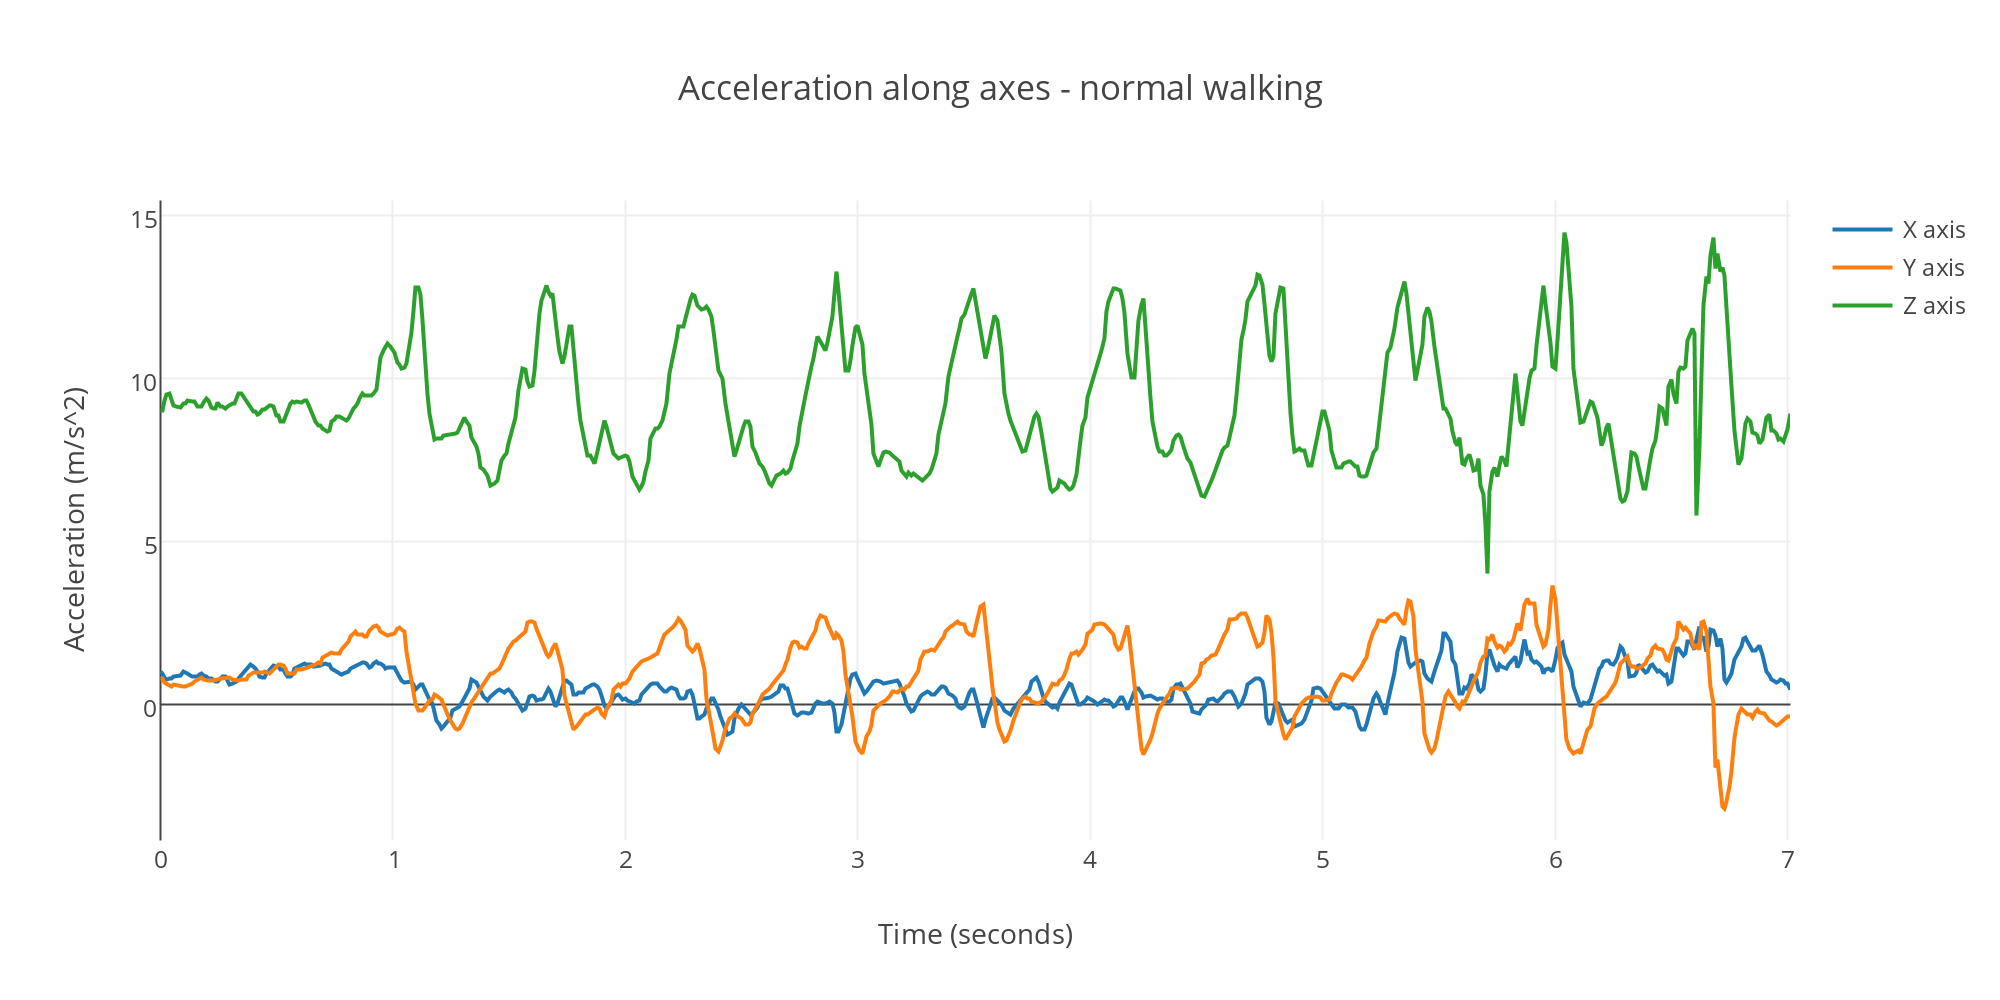
\includegraphics[scale=0.9]{images/straightWalkRaw.png}
\captionof{figure}{Accelerometer readings during normal walking}
\label{fig:straightWalkRaw}
\end{center}

As observed in the figure there is a periodic rise and fall in both the Y-axis and Z-axis accelerometer readings, while the X-axis readings do not exhibit much variation and remain close to 0 throughout. This is because when the phone is kept in the hand in portrait mode the majority of the gravity component is split vertically among the Y and Z axes, while there is negligible horizontal acceleration.

The periodicity in the Y and Z readings corresponds to the two phases of walking motion - the user beginning their step by lifting their foot off the surface followed by completing the step with bringing their foot down to make contact with the surface again. The first phase causes the phone to accelerate vertically along the direction of gravity acceleration as the user moves upwards. These are represented as peaks in the graph as the accelerations add together. In the second phase the user moves downwards and thus accelerates in a direction opposite to that of the gravity acceleration, leading to the formation of the valleys in the graph. Thus each peak/valley combination can be associated with individual steps, potentially allowing step identification to be carried out by detecting peaks and valleys in the graph generated by the accelerometer readings. This notion is supported by the plot in Figure~\ref{fig:straightWalkRaw}, where there are roughly 10 peak/valley pairs for both the Y and Z readings corresponding to the 10 steps taken.   

The primary issue with this approach is that step detection is dependent on the orientation in which the phone is kept. For instance, if the user holds the phone in landscape mode instead of portrait then a major component of the acceleration will  be along the X axis. This makes it difficult to keep track of periodic changes in acceleration as variations along all the three axes must be considered simultaneously depending on the phone's orientation. This problem is overcome by computing the magnitude of the accelerometer vector and using that instead to detect steps. The magnitude combines the acceleration information from the three axes into a single scalar quantity, which by definition, is independent of direction and makes it robust to changes in orientation. The magnitude plot of the acceleration values in Figure~\ref{fig:straightWalkRaw} is provided in Figure~\ref{fig:straightWalkRawMagnitude}. 

\begin{center}
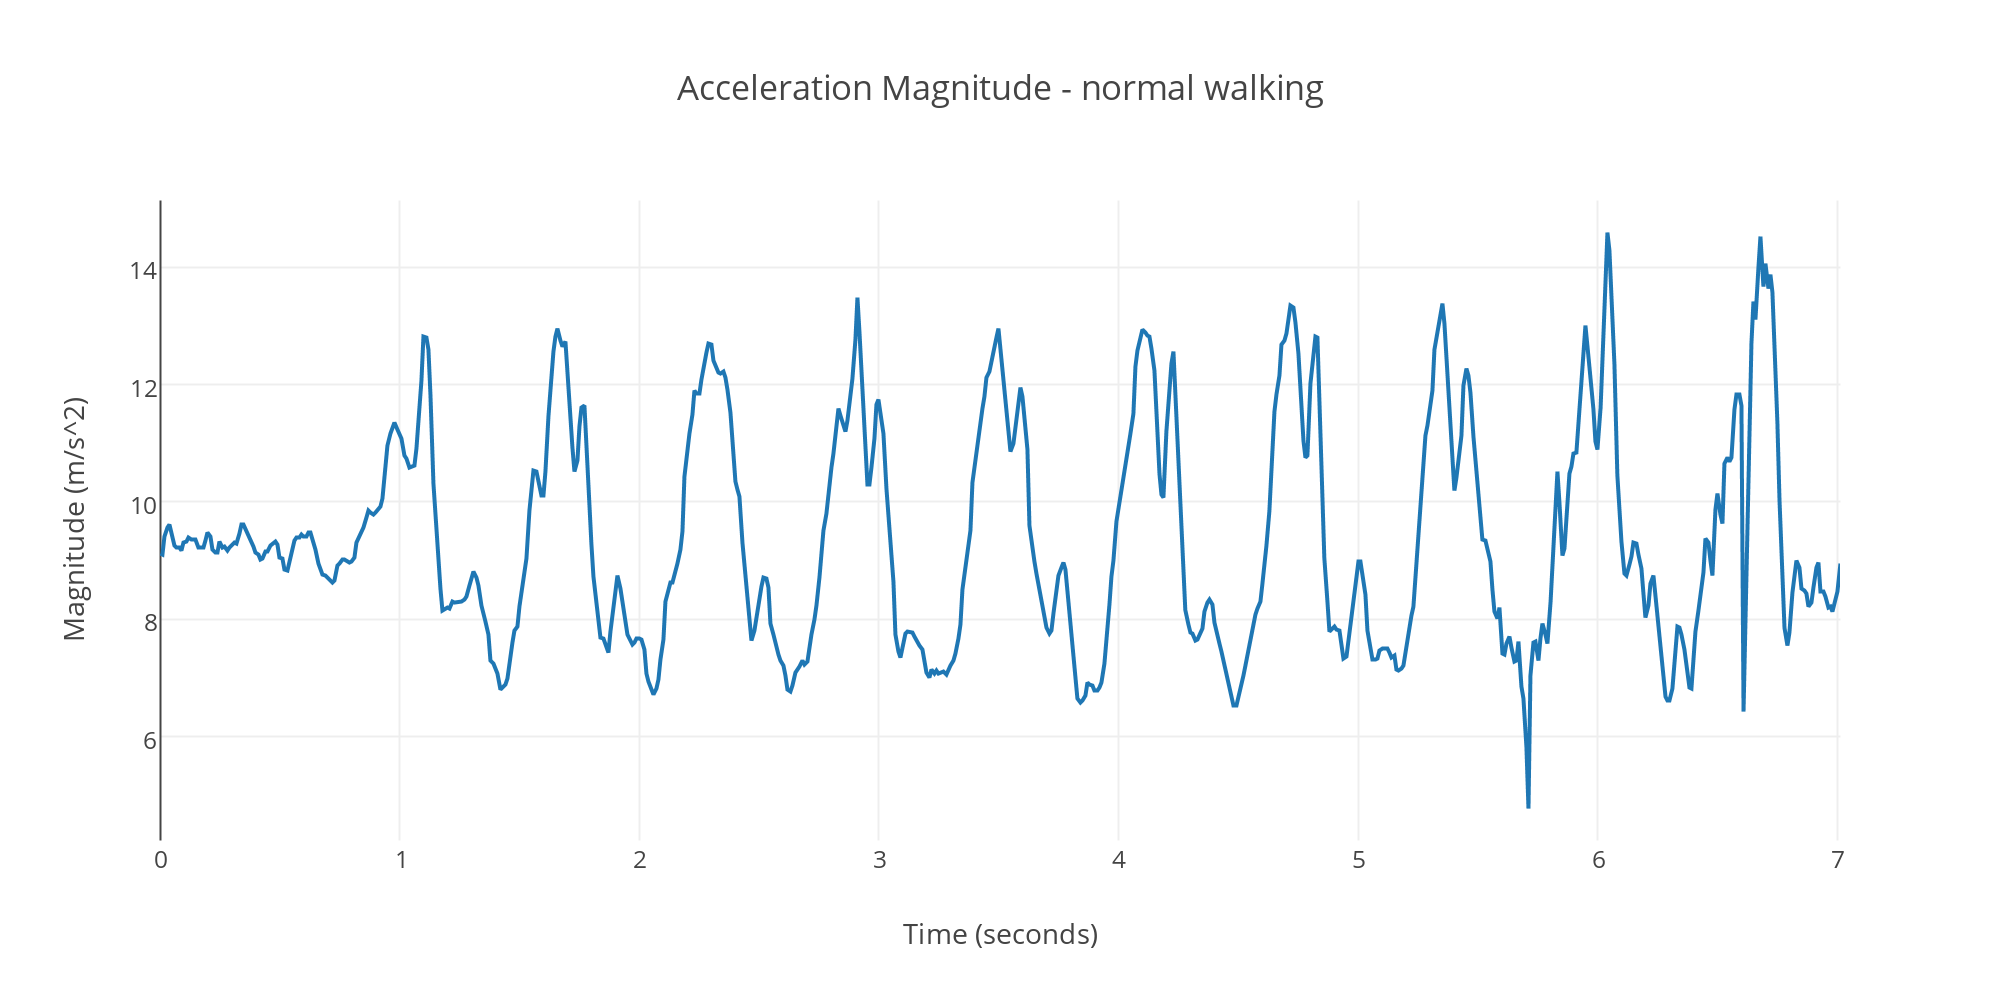
\includegraphics[scale=0.9]{images/straightWalkRawMagnitude.png}
\captionof{figure}{Accelerometer magnitude during normal walking}
\label{fig:straightWalkRawMagnitude}
\end{center}

From the plot it can be seen that using magnitude still preserves the 10 peak/valley pairs corresponding to steps that were identified in the previous graph. Thus step detection can now be carried out on the basis of a single measure that accounts for changes in orientation. 


\nocite{*}

\bibliography{StepDetection}
\bibliographystyle{plain}

\end{document}